\documentclass[11pt,a4paper]{article}
\usepackage[english, ngerman]{babel}
\usepackage[autostyle]{csquotes}
\usepackage{natbib}
\usepackage{hyperref}
\usepackage{graphicx}
\usepackage{subcaption}
\usepackage[raggedrightboxes]{ragged2e}
\usepackage{pgf-pie}
\usepackage{pgfplots}
\usepackage[acronym, toc, numberedsection]{glossaries}
\usepackage{pgfplots}

\makenoidxglossaries
\newacronym{bs}{BS}{Radio Base Station}
\newacronym{ue}{UE}{User Equipment}
\newacronym{m2m}{M2M}{Machine-to-Machine}
\newacronym{lte}{LTE}{Long-Term Evolution}
\newacronym{nsa}{NSA}{Non-standalone}
\newacronym{3g}{3G}{3\textsuperscript{rd} generation mobile network}
\newacronym{4g}{4G}{4\textsuperscript{th} generation mobile network}
\newacronym{5g}{5G}{5\textsuperscript{th} generation mobile network}
\newacronym{6g}{6G}{6\textsuperscript{th} generation mobile network}
\newacronym{aau}{AAU}{Active Antenna Unit}
\newacronym{bbu}{BBU}{Building Baseband Unit}
\newacronym{rru}{RRU}{Remote Radio Unit}
\newacronym{ac}{AC}{Air Conditioning}
\newacronym{cu}{CU}{Centralized Unit}
\newacronym{du}{DU}{Destributed Unit}
\newacronym{nrl}{NR-Light}{New Radio Light}
\newacronym{redcap}{RedCap}{Reduced Capability NR}
\newacronym{nr}{NR}{New Radio}
\newacronym{d2d}{D2D}{Device-to-Device}
\newacronym{n2d}{N2D}{Network-to-Device}
\newacronym{dl}{DL}{Downlink}
\newacronym{ul}{UL}{Uplink}
\newacronym{cpu}{CPU}{Central Processing Unit}
\newacronym{wifi}{WiFi}{Wireless Fidelity}
\newacronym{mimo}{MIMO}{multiple-input and multiple-output}

\makeatletter         
\renewcommand\maketitle{
{\raggedright
\begin{center}
{\Large \bfseries \@title}\\[2ex] 
\@author\\[1ex] 
\@date, Hochschule der Medien, Stuttgart\\[1ex]
\end{center}}} 
\makeatother

\bibliographystyle{plainnat}

\title{Energy Footprint of Mobile communications in the 21\textsuperscript{st} century}
\author{Andreas Nicklaus}

\begin{document}
\maketitle

\begin{abstract}
  Diese Arbeit untersucht die Umweltbelastung des Mobilfunks im 21. Jahrhundert, wobei der Schwerpunkt auf Deutschland liegt.
  Seit dem Aufkommen von Mobilfunktechnologien, insbesondere mit der Verbreitung von Smartphones und dem Übergang zu 4G- und 5G-Netzen, ist der Energieverbrauch von Basisstationen und Nutzergeräten deutlich gestiegen.
  Durch eine Analyse der nationalen Energiedaten, der Dynamik der Basisstationen und der Trends bei den Nutzergeräten beleuchtet das Papier die Umweltauswirkungen der Mobilfunktechnologien.
  Zu den wichtigsten Erkenntnissen gehören der beträchtliche Beitrag erneuerbarer Energiequellen zur Stromerzeugung, der Energiebedarf der Komponenten von Basisstationen und die Herausforderungen bei der Schätzung des Stromverbrauchs von Nutzergeräten.
  Das Papier zeigt auch Möglichkeiten zur Energieeinsparung auf und betont die Bedeutung nachhaltiger Praktiken bei der Abschwächung der Umweltauswirkungen der mobilen Kommunikation.
  Um energieeffiziente und umweltverträgliche Mobilkommunikationssysteme voranzutreiben, sind weitere Forschung und Zusammenarbeit unerlässlich.
\end{abstract}

\selectlanguage{english}
\begin{abstract}
  The paper investigates the energy footprint of mobile communications in the 21\textsuperscript{st} century, with a focus on the context of Germany.
  Since the advent of mobile communication technologies, especially with the proliferation of smartphones and the transition to 4G and 5G networks, there has been a significant increase in energy consumption associated with base stations and user equipment.
  Through an analysis of national energy data, base station dynamics, and user equipment trends, the paper sheds light on the environmental implications of mobile communication technologies.
  Key findings include the substantial contribution of renewable energy sources to electricity production, the energy demands of base station components, and the challenges in estimating the power consumption of user equipment.
  The paper also identifies opportunities for energy saving and emphasizes the importance of sustainable practices in mitigating the environmental impact of mobile communications.
  Moving forward, continued research and collaboration are essential for advancing energy-efficient and environmentally responsible mobile communication systems.
\end{abstract}

\noindent\textbf{Dislaimer:} This paper has been written with the help of AI tools for translating sources and outlining parts of the written content.
All content has been written or created by the author unless marked otherwise.

\tableofcontents

\section{Introduction}\label{sec:intro}
% Vision: why and what is this topic?
Since around 2010, mobile communication has been a vital part of everyday-life for most of the western world.
In 2007, we saw the launch of the iPhone, arguably one of the most influencial inventions in the mobile market ever.
With the introduction of \acrfull{4g} in late 2009 came a massive increase in mobile communication over the internet.
For almost one and a half decades, more and more technology has been invented for the mobile phone market.

In addition, the Oculus Rift has ushered in the reincarnation of the idea of Virtual Reality and spacial computing, plainly meaning the usage of 3D-space as a way to distribute user interfaces.
More and more, we rely on small, wireless devices with a sleek, modern and fashionable design and people seem to keep buying in. 
With that in mind, most mobile \acrfull{ue} has had one spatial constraint that has so far never been overcome: Battery life and usage breaks to recharge at a wall socket.
This paper focuses on the effectiveness of energy consumption in respect to the overall environmental impact of modern mobile communications.
To this end, the following chapter~\ref{sec:relatedwork} summarizes other work done in the field and its topics.
Chapter~\ref{sec:energyfootprint} introduces a definition of environmental footprint and its relevance to this topic.
The chapters~\ref{sec:influence} and~\ref{sec:energyconsumption} go into detail about the energy production and consumption in Germany both in general and related to mobile communications.
Chapter~\ref{sec:opportunities} then names a few opportunities for saving energy.

\section{Related Work}\label{sec:relatedwork}
% What sources have the same or similiar topic?

% Öffentliche Zahlen und Angaben
% - Bruttostromerzeugung bis 2022 \cite{Bruttostromerzeugung2022}
% - Umweltindikatoren \cite{Umweltindikatoren}
When inspecting the relevance of mobile communications within the global energy market, one can only rely on data given out by nations or leagues of nations.
\citep{Stromverbrauch} gives a summary of the electricity consumption in Germany by year and \citep{Bruttostromerzeugung} shows the production of electrical power between 2019 and 2022 by energy source.

\citep{Umweltindikatoren} lists generalized indicators for environmental impact.
These indicators are meant to help analyze the effect of any product or project on the environment.

% 5G Power Whitepaper \cite{powerwhitepaper}
% - insights into the power consumption of parts of base stations
% - challenges in site power construction
% - pointers to the meaning of efficient energy saving strategies
The whitepaper \citep{powerwhitepaper} is a technical report on the state of \acrfull{bs} and gives insight into the power consumption of \acrshort{bs} as a whole and parts.
The paper also outlines challenges for the construction of site power supply and gives pointers to what efficient power saving strategies could do.

% 5G Energy Efficiency \cite{5GEfficiencyOverview}
% - describes the energy consumption and efficiency of base stations in detail
% - power consumption of switching between sleep mode an active state
\citep{5GEfficiencyOverview} describe the energy consumption and efficiency of \acrshort{bs} in detail and examines the power consumption of switching between a sleep state and an active state.

% Dynamic gNodeB Sleep Control fo rEnergy-Conserving 5G Radio Access Network \cite{DynamicSleepModeControl}
% - outlines the changes between 4G and 5G
% - proposes sleep mode switching policies
% - comparison
\citep{DynamicSleepModeControl} outline the technical changes going from \acrshort{4g} to \acrfull{5g} infrastructure.
Based on those findings, they propose multiple sleep mode switching policies and gives a comparison between them.

\section{Environmental footprint}\label{sec:energyfootprint}
% What does it mean here?
This chapter gives an outline of the meaning of environmental impact and the metrics for it.
First, the section~\ref{subsec:indicators} summarizes the indicators factoring into the effect on the environment.
Second, the section~\ref{subsec:relevancy} gives first answers to the relevancy of those indicators and interprets why some indicators are more relevant to this topic than others.

\subsection{Indicators for environmental footprint}\label{subsec:indicators}
% Of what does energy footprint consist?
% Categories
% Indicators

When we want to analyze the impact something has on the environment, we need to have consistent metrics to give values to and compare.
\citep{Umweltindikatoren} gives 27 general indicators as to what those metrics have to reflect on and are grouped into four categories.
Table~\ref{tab:indicators} show all indicators within its category.

\begin{table}[t]
  \centering
  \begin{tabular}{p{0.21\linewidth}|p{0.21\linewidth}|p{0.21\linewidth}|p{0.21\linewidth}}
    \textbf{Climate and Energy} & \textbf{Nature and landscape} & \textbf{Environment and health} & \textbf{Resources and efficiency}\\
    \hline
    Climate change and vegetation development & Landscape fragmentation & \textit{Air quality} & Waste generation\\
    \hline
    \textit{Carbon dioxide emissions} & Species diversity and landscape quality & \textit{Noise pollution} & \textit{Recycling rate}\\
    \hline
    \textit{Energy consumption} & Red List species & Road traffic noise & \textit{Resource productivity}\\
    \hline
    \textit{Renewable energies} & Area for nature conservation objectives & Freight transport performance & Organic farming\\
    \hline
    & Agricultural land with high nature value & Local public transport & \textit{Settlement and traffic area}\\
    \hline
    & Forest condition & Nitrate in groundwater & \textit{Land use}\\
    \hline
    & Acidity and nitrogen input & Heavy metal input & \textit{Contaminated sites}\\
    \hline
    & Nitrogen surplus &\\
    \hline
    & Ecological status of surface waters &\\
  \end{tabular}
  \caption{27 Environmental Indicators \citep{Umweltindikatoren}, italics are relevant to mobile communications}
  \label{tab:indicators}
\end{table}

For this paper, these indicators will be used to narrow down the topic down to the most relevant factors.

\subsection{Relevancy of indicators}\label{subsec:relevancy}
% Values for the first indicators
% What will be the topic of the rest of the chapters

On the topic of mobile communications in general, all indicators of the category \enquote{Nature and landscape} can be ignore due to the fact that they are not applicable to either \acrshort{bs}, cable laying to and from those \acrshort{bs} or the \acrshort{ue}.

From the category \enquote{Climate and Energy}, the indicator Climate change and vegetation development will be ignored due to the \acrshort{bs}' signal outputs' unproven significance on the vegetation.
The effect of \acrshort{bs} on the climate change is only noticable through the usage of electicity which is inspected under the other indicators of the category.

The category \enquote{Environment and health} only yields the relevant indicators air quality and noise pullution, both mainly dependent on the energy source of \acrshort{bs} and \acrshort{ue}.
The other indicators of the category will be ignore because they are not applicable to mobile communications.
The positive effect that mobile communications might have towards the management of traffic and both freight and public transport are not inspected in this paper.

Preliminary tests of eight \acrlong{bs}s in Eislingen/Fils, Germany, have shown that none of the examined systems contribute to audible noise pollution.
Five \acrshort{bs}s have been measured with environment noise.
These measurements show an average of approximately 40 dBA with an average distance to the antenna systems of 22 meters.
Figure~\ref{fig:noise-measurements} shows the minimal, maximal and average noise level of those measurements.
Although all units are visible from street level and some have a maximum noise level that would be descernible from background noise, all measurements above 50 dbA are caused by their location, e.g. industry buildings or a train station.
No units reach a noise level above 60dbA.
Based on this data, noise pollution is considered no factor in the environmental impact of \acrlong{bs}s.

\pgfplotstableread[row sep=\\,col sep=&]{
    unit & 751424  & 27012311 & 752135 & 750340 & 275186 \\
    min.  & 40      & 26.5     & 29.2   & 37.2   & 40.8 \\
    avg.  & 49.9    & 27.5     & 31.5   & 46.2   & 43 \\
    max.  & 58.6    & 30.4     & 33.8   & 54.2   & 47.6 \\
    }\noiseData

\begin{figure}[h]
  \centering
  \begin{tikzpicture}
    \begin{axis}[
            ybar,
            % ymax=300,
            symbolic x coords={min., avg., max.},
            xtick=data,
            % nodes near coords,
            bar width=.25cm,
            enlarge x limits=0.3,
            % enlarge y limits=0.3,
            legend style={
              at={(1.5,1)},
              anchor=north,
              legend columns=1
            },
            % ylabel={dbA},
            width=.6\textwidth,
            % height=.35\textwidth,
        ]
        \addplot table[x=unit,y=27012311]{\noiseData};
        \addplot table[x=unit,y=752135]{\noiseData};
        \addplot table[x=unit,y=275186]{\noiseData};
        \addplot table[x=unit,y=750340]{\noiseData};
        \addplot table[x=unit,y=751424]{\noiseData};
        \legend{
          Lerchenweg 2 (27012311),
          Vogelgartenstr. 10 (752135),
          Teckstr. 4 (275186),
          Ulmer Str. 46 (750340),
          Schillerstr. 23-25 (751424),
        }
    \end{axis}
  \end{tikzpicture}
  \caption{Noise levels of measured \acrshort{bs}s in 70354 Eislingen/Fils, Germany. The legend includes the \enquote{Standortbescheinigungs-Nr.} of the unit~\citep{EMFKarte}. \enquote{Teckstr. 4} is the only radio tower.}\label{fig:noise-measurements}
\end{figure}

This paper assumes that only a insignificant number of \acrshort{bs} are built on agricultural land and that once built these \acrshort{bs} produce next to no waste at all.
Therefore the indicators waste generation and organic farming can be left out of this paper.
All other indicators from the category \enquote{Resources and efficiency} are applicable to the build site and lifecycle of \acrshort{bs} and \acrshort{ue} and are applicable to mobile communications.


The indicators \enquote{Carbon dioxide emissions}, \enquote{Air quality} and \enquote{Noise pollution} all boil down the source of electical power of the base station and \acrshort{ue}.
\citep{powerwhitepaper} implicates that near all \acrshort{bs} use whatever electical power they can get on-site and have lithium-ion batteries for emergency-power.
With that electrical equipment the effect of those three indicators are dependent on the source on the power grid and therefore dependent on the indicators \enquote{Energy consumption} of the equipment and the \enquote{Renewable energies} produces for the power grid of the region.

\enquote{Settlement and traffic area}, \enquote{Land use} and \enquote{Contaminated sites} come down the the area that build site of  \acrshort{bs}.
\citep{BSStandort} states in its advertisement for new build site of \acrshort{bs} \enquote{Around ten square meters of technical space is required to operate a radio station on the roof, and around 150 square meters of floor space or technical space is required for a mast}.
Because it is possible to use already developed areas and effect on the above mentioned indicators is not caused by the building of new \acrshort{bs}, the effect of \acrshort{bs} can be considered nonexistent.

This means that only four of the 27 indicators are relevant to mobile communications:
\begin{enumerate}
  \item \textbf{Energy consumption}: Energy, electrical and other, consumed per consumer unit and consumption time. Usually measured in kWh per person and year.
  \item \textbf{Renewable energies}: Share of renewable energy in energy consumption and production (assumed to be equal here).
  \item \textbf{Recycling rate}: Share of recycled materials in total waste generation.
  \item \textbf{Resource productivity}: Ratio of gross domestic product to primary energy consumption or raw material consumption in relation to a base year.
\end{enumerate}

The upcoming chapters will only cover the energy consumption and share of renewable energies because the recycling rate and resource productivity outgrow the scope of this paper.

\section{Numbers: mobile communication and national power consumption}\label{sec:influence}
% Narrowing down the topic "environment" to "energy and power" to electricity
% Specifying Germany as the investigated region

Having narrowed down the topic of environmental impact of mobile communications down to the power consumed by the equipment and the resources used in production and after usage, this chapter aims to give comparison and numbers filling in the indicators of chapter~\ref{sec:energyfootprint}.
For the comparison, the assumption is made that the usage and production of base stations is similiar around the world although for the energy consumption and production, the mobile communications and energy markets of only Germany will be inspected. 

\subsection{National energy data of Germany}\label{subsec:nationalaverage}
% What is the national power consumption and production in Germany?
In the year 2022, 573.1 TWh of electricity were produced gross, close to 2\% less than the three-year average of ca. 584.06 TWh in 2019-2022.
Of that, 254 TWh (44\%) were produced using renewable energy sources, mainly wind power and photovoltaics \citep{Bruttostromerzeugung}.
Over the whole year 2022, 11,01\% (63,1 TWh) of the greed feed-in were imported \citep{energieErzeugung}.
In the third quartal of 2022, 10.99\% (13 of 118.2 TWh) have been imported and 16 TWh have been exported.
The third quartal of 2023 showed an increase of imported feed-in to 23.1 TWh and 9.9 TWh exported power \citep{stromerzeugung3Quartal2023}.

In 2022, 552 TWh have been consumed gross \citep{Stromverbrauch} and 490.6 TWh net \citep{NettoStromverbrauch}.
Of the gross consumption, 46\% have been from renewable energy sources \citep{Stromverbrauch}.

\subsection{Base Stations}\label{subsec:BSInfluence}
% How much do the base stations consume?
% Juli 2023: 89% Abdeckung
% 3kW pro BS
% 14200 Standorte (Telekom)
% 41.945 Basisstationen (2022) laut Statista https://de.statista.com/statistik/daten/studie/1237437/umfrage/anzahl-der-5g-basisstationen-in-deutschland/
% 71510 Mobilfunkstandorte in Deutschland: https://www.bundesnetzagentur.de/DE/Fachthemen/Telekommunikation/Technik/EMF/start.html
% 42% 6 oder mehr, 14% 5, 8% 4, 12% 3, 13% 2 und 10% eine Mobilfunkanlage https://www.bundesnetzagentur.de/SharedDocs/Downloads/DE/Sachgebiete/Telekommunikation/Verbraucher/ElektromagnetischeFelder/Statistiken/standortmitbenutzung_20240101.pdf?__blob=publicationFile&v=1
%   inklusive:LTE 800 MHz, GSM 900 MHz, GSM/LTE 1800 MHz, UMTS/LTE 2600 MHz, 5G 3600 MHz

According to \cite{BSStandort}, a build-site for single \acrshort{bs} needs a power supply that can deal with a constant load of 3kW.
In \cite{vodafoneAusbau}, Vodafone states to have have built 14200 sites with at least some \acrshort{5g} capabilities and there are 41945 \acrshort{5g} \acrlong{bs}s in Germany \citep{5gBS}.
The exact number of \acrshort*{bs} is probably difficult to determine because there are only very few public technical reports on the expansion to \acrshort{5g} and most of the marketing publications online have no technical information as to which \enquote{\acrshort{5g} \acrlong{bs}s} include sites with \acrfull{lte} functionality used for \acrfull{nsa} mode \acrshort{5g} New Radio.

\begin{figure}[h]
  \centering
  \begin{tikzpicture}
    \pie[sum=auto, after number=\%, radius=2, text=legend]{42/6 or more radio systems, 14/5 radio systems, 8/4 radio systems, 12/3 radio systems, 13/2 radio systems, 10/1 radio system}
  \end{tikzpicture}
  \caption{Distribution of radio systems within all \acrlong*{bs} sites in Germany \citep{EMF} (missing one percent due to rounding errors)}
  \label{fig:EMFdistribution}
\end{figure}

However, it is known that there are 71510 \enquote{mobile phone sites} in Germany.
This number includes radio sites with \acrshort{lte} (800 MHz), GSM (900 MHz), GSM/\acrshort{lte} (1800 MHz), UMTS/\acrshort{lte} (2600 MHz) and \acrshort{5g} (3600 MHz) equipment.
Figure~\ref{fig:EMFdistribution} shows the distribution of number of radio systems on those sites \citep{EMF}.

Taking 41945 \acrshort{5g} \acrlong{bs}s and 3kW as our reference number of units and power consumption for \acrshort{5g} under full load, it can be estimated that the total grid load is 125.835 GW.
Assuming full load all year around the maximum power consumption can be calculated with 1.1023146 TWh per year or 26.28 MWh per site and year.
This results in 0.19969\% of the gross and 0.224687\% of the net national power consumption.
0.19234\% of the national electrical power production is used up by the base stations in the Germany.

Note that the number of \acrshort{5g} base stations in 2022 was enough to \enquote{only} cover 79\% of the nation's area \citep{5Gausbau}.
To adapt for a complete coverage in the future, the number of the above paragraph will be multiplied by factor of 1.266 (overlap not included).
Also, this calculation assumes a full usage of the power supply at all times without idle time or down time.

\subsection{User Equipment}\label{subsec:UEInfluence}
% What percentage of the national power consumption / production is that? 
% 169 Millionen Mobilfunkanschlüsse in Deutschland https://de.statista.com/statistik/daten/studie/3907/umfrage/mobilfunkanschluesse-in-deutschland/
% 8.59 Milliarden Mobilfunkanschlüsse in der Welt https://www.weforum.org/agenda/2023/04/charted-there-are-more-phones-than-people-in-the-world/
% 6,93 Milliarden Smartphonenutzer, 7,41 Milliarden Mobiltelefonnutzer in 2024 https://www.bankmycell.com/blog/how-many-phones-are-in-the-world
% 2022: 67.6 Mio Smartphonenutzer in Deutschland https://de.statista.com/statistik/daten/studie/198959/umfrage/anzahl-der-smartphonenutzer-in-deutschland-seit-2010/
% 2022: 124 Pro 100 Mobilfunkanschlüsse ohne M2M https://de.statista.com/statistik/daten/studie/13264/umfrage/penetrationsrate-der-deutschen-mobilfunknetze-seit-1990/
% 2022: 104,904 Mio. Mobilfunkanschlüsse ohne M2M (62,07%; 84,6 Mio. Einwohner) https://www.destatis.de/DE/Themen/Gesellschaft-Umwelt/Bevoelkerung/Bevoelkerungsstand/_inhalt.html
% 2022: 75,5 Mio. LTE-fähige SIM-Karten (44,67%) https://de.statista.com/statistik/daten/studie/974622/umfrage/anzahl-der-aktiven-lte-faehigen-sim-karten-in-deutschland/
% Erstes 5G-Smartphone März 2019 https://www.yourfone.de/mobilfunk-ratgeber/5g-handys
% Seit Beginn 2019 87,9 Mio. Smartphones verkauft (2022 21,6 Mio., 2021 22,2 Mio., 2020 22 Mio., 2019 22,1 Mio.), Anteil der 5G-Handys unbekannt https://blogs.fu-berlin.de/hci2023/files/2023/05/study_id71707_smartphone-nutzung-in-deutschland.pdf
% durchschnittlich 10 Wh pro Ladevorgang -> 3,65 kWh im Jahr https://www.gasag.de/magazin/energiesparen/stromverbrauch-smartphone
% 5G-Tablets seit Nov. 2021 (Verkaufszahlen unbekannt), 19 Modelle in Deutschland https://www.vodafone.de/featured/smartphones-tablets/5g-tablets-apple-samsung-beste-modelle/#/
% 3 5G-Laptop Modelle in Deutschland https://www.5g-anbieter.info/hardware/laptops-mit-5g.html
% keine Daten zu Modellen und Verkäufen von 5G-fähigen Wearables etc.
% Annahme: Smartphones bilden guten Durchschnitt für UE
% Rechnungen mit 169 Millionen und 104,904 Mio. Endgeräten
As for the \acrlong{ue}, two categories will be differentiate between in this paper: devices actively used by humans and \acrfull{m2m} communications.
There are 8.59 billion mobile phone subscriptions~\citep{mobilephonesWorld} and 7.41 billion mobile phone users, of which 6.93 billion are smartphone users \citep{mobileusersWorld}.

In Germany, the number of smartphone users in 2022 was 67.6 million \citep{smartphonenutzerDeutschland}, but there have been 104,904 million mobile phone subscriptions (124 per 100 capita \citep{mobilesubscriptionsDeutschland}) for the 84.6 million people living in Germany \citep{consensusDE2022}.
That only describes the mobile phone subscriptions for human-used devices.
The total count of subscriptions including \acrshort{m2m} devices is 169 million \citep{totalmobilesubscriptionsDeutschland}, meaning about 37.93\% of mobile communication connections are \acrshort{m2m} communication.
These number describe the total number of SIM-cards in Germany without specifying wether or not the activity coming from those connections classify as \enquote{modern}.
Only 44.67\% of the total number of SIM-Cards in circulation in Germany (77.5 million \citep{simCardsDeutschland}) have some form of \acrshort{lte} functionality (see Figure~\ref{fig:simdistribution}).

\begin{figure}[t]
  \begin{tikzpicture}
    \pie[sum=auto, after number={\space M}, radius=1.7, text=legend, color={violet!60, green}]{64.096/SIM-cards in \acrshort{m2m} devices (37.93 \%), 104.904/SIM-cards in human-used devices (62.07 \%)}
  \end{tikzpicture}

  \begin{tikzpicture}
    \pie[sum=auto, after number={\space M}, radius=1.7, text=legend, color={orange, yellow}]{77.5/SIM-cards with \acrshort{lte} capabilities (44.67 \%), 93.5/SIM-cards without \acrshort{lte} capabilities (55.33 \%)}
  \end{tikzpicture}

  \caption{Distribution of SIM-cards in Germany between \acrlong*{m2m} and human-used devices and between cards with and without \acrshort{lte} capabilities (\acrshort{lte} or more modern), totaling 169 million (M) cards}
  \label{fig:simdistribution}
\end{figure}

When it comes to the devices used for mobile communication, the situation is opaque.
Very little is known about the devices in use and their specifications in \acrshort{m2m} communication (47.93\%).
There only is some information of human-used devices that helps estimate the number of eligable and active devices.
The first smartphone with \acrshort{5g} capabilities entered the German market in march of 2019 \citep{smartphonemodells5G}.
Since the beginning of 2019, 87.9 million smartphones have been sold in Germany until 2022 (22.1 million in 2019, 22 million in 2020, 22.2 in 2021 and 21.6 million in 2022) \citep{smartphonenutzungDeutschland}.
The share of smartphones with \acrshort{5g} capabilities is unknown.

The number of other human-used devices is about as opaque as the \acrshort{m2m} devices.
It is known that there have been only 19 models of \acrshort{5g}-capable tablets in the German market (beginning in November 2021) \citep{tabletmodels} and 3 \acrshort{5g}-capable laptop models \citep{laptopmodels}.
The number of other \acrlong{ue}, e.g. wearables, remains unclear.

All this makes the calculation of the power demand by \acrlong{ue} very difficult.
It is not possible to make a reliable and accurate statement about the power consumption for those devices.
However, it is possible to make an estimation under some assumptions.
Firstly, the assumption will be made that the average power consumption of modern smartphones is a good estimation for the power consumption of any \acrshort{ue}.
In order to reconsile with this assumption two calculations will be made: One for all devices and one only for human-used devices.
Secondly, the share of SIM-cards with/without \acrshort{lte} capability remains a constant throughout the \acrlong{ue} space, meaning the share of 44.67\% can be used across all devices types.
This seems a good assumption because it is unclear with the currently available information to know more about the actual situation and it seems improbable that all 64.096 million \acrshort{m2m} devices have SIM-cards with \acrshort{lte} capabilities, leaving only 11.404 million for human-used devices.


With those assumptions established and the information that the charging of a smartphone consumes an average of 3.65 kWh per year (10 Wh per over-night charge for 365 days per year) \citep{smartphonecharge}, the estimation of the power consumption of \acrshort{ue} is as follows:
The 104.904 million human-used devices in Germany consume 382.8996 GWh per year and the total 169 million \acrshort{ue} devices in Germany consume 616.85 GWh per year.
Of those, we are only concerned with the devices participating in modern mobile communications (44.67\%), bringing those numbers down to 171.041 and 275.547 GWh respectively.

\section{Sources of energy consumption}\label{sec:energyconsumption}
In order to outline the opportunities for saving energy, this chapter gives details about what parts of \acrlong{bs}s and \acrlong{ue} consume most of the power.
The following chaper~\ref{sec:opportunities} then describes five technologies that either increase efficiency or save power entirely.

\subsection{Base Stations}\label{subsec:BSConsumption}
% What is in a base station?
% What parts are responsible for most of the power consumption

The parts of a modern \acrshort{bs} can be seperated into several units.
The antenna system and \acrfull{rru} are capable of convertimg and sending a baseband signal as a radio signal and the \acrfull{bbu} modulates a signal from and onto the used radio frequency.
The physical support system includes all components to keep the antenna system, \acrshort{rru} and \acrshort{bbu} running, e.g. the power supply, backup batteries, transmittion equipment like cables and converters and \acrfull{ac}.
Due to the current situation, in which the \acrshort{bbu}s can have some distance to the antenna systems and \acrshort{rru} and can supply more than one, the antenna system and \acrshort{rru} are often combined to a \acrfull{aau} and \acrshort{bbu}s are differentiated between \acrfull{cu} and \acrfull{du}.

\begin{figure}[h]
  \centering
  \begin{tikzpicture}
    \begin{axis}[
      xlabel=Traffic Load,
      ylabel=Avg. Power Consumption (W),
      xmin=0, xmax=100,
      xticklabels={0\%, 25\%, 50\%, 75\%, 100\%},
      xtick={0, 25, 50, 75, 100},
      legend style={at={(.5,1.15)}, draw=none, anchor=north, legend columns=-1},
      ]

      \addplot[smooth,mark=*,blue] plot coordinates {
        (0,650)
        (10,720)
        (20,767.5)
        (30,812.5)
        (50,932.5)
        (100,1155)
        };
      \addlegendentry{AAU}
      
      \addplot[dashed, blue] plot coordinates {
        (0,175)
        (100,175)
        };
      \addlegendentry{AAU Deep Sleep}

      \addplot[smooth,mark=*,red] plot coordinates {
        (0,307.5)
        (10,307.5)
        (20,307.5)
        (30,307.5)
        (50,307.5)
        (100,307.5)
        };
      \addlegendentry{BBU}
      
      \addplot[dashed, red] plot coordinates {
        (0,307.5)
        (100,307.5)
        };
      \addlegendentry{BBU Deep Sleep}

      \addplot[orange] plot coordinates {
        (0,1740)
        (100,1740)
        };
      \addlegendentry{AC}
    \end{axis}
  \end{tikzpicture}
  \caption{Average power consumption of  \acrshort{aau}, \acrshort{bbu} and \acrshort{ac} by traffic load and its respective deep sleep power consumption \citep{green5G}}
  \label{fig:BSConsumption}
\end{figure}

Figure~\ref{fig:BSConsumption} shows the power consumption by \acrshort{bs} unit and traffic load and the power consumption of each unit in a deep sleep mode.
The power consumption of the the \acrshort{ac} is shown seperately from the other physical support equipment because the rest has a power consumption of next to zero.  
Note that the power consumption of the \acrshort{bbu} and the \acrshort{ac} are static and more importantly independent from the traffic load.
For the \acrlong{ac}, \acrlong{bs}s have the specific demand of disabling the \acrshort{ac} on low traffic times or when the environment is cold anyways, which is sensible.
On the other hand, the demand for power saving to be dependent on traffic load usually concerns short time intervals, e.g. few milliseconds or seconds, which is shorter than the average reaction or effect time of a \acrlong{ac} unit.

Because this seems obvious and managable during research, the question is raised whether this can be true.
During research, no answer was found on this question and no operator of \acrshort{bs} was willing to answer questions.

\subsection{User Equipment}\label{subsec:UEConsumption}
% What parts are responsible for most of the power consumption
% CPU: 500-2000 mW (Peak 3000 mW) or 55 - 612 mW depending on usage
% Display: 400 or 1000-1500 mW or 63 - 527.05 mW depending on usage (13.86 mW in screensaver mode)
% Active cell radio: 800 mW
% Bluetooth: 100 mW (Usage: 12 - 432 mW)
% Accelerometer: 21 mw
% Gyro: 130 or 25 mW
% Mircrophone: 101 mW
% GPS: 176 or 25 mW
% Camera up to 1000mW
% Data Writing: 400 or 580 mW per MB (avg)
% Downloading through WiFi @4.5Mbps: 1450 mW
% 3G Downaload @1Mbps: 1400 mW
% 3G voice call: 1224.3 - 1265.7 mW

The power consumption of a modern smartphone varies largely based on the used hardware parts and software optimizations.
While some sources from the past decade claim the power usage of a \acrshort{cpu} to vary between 500 and 2000 mW \citep{smartphoneEnergyConsumption}, other sources see these numbers between 55 and 612 mW \citep{smartphoneEnergySurvey} or 5.1 nd 11.1 mW \citep{mobileEnergyConsumption} (note that different \acrshort{cpu} models were used in the sources).
This discrepency continues with other components like the display (400 mW on average \citep{smartphoneEnergyConsumption}, 1000-1500 mW \citep{powerUsageSmartphonesQnovo} or 63-527.05 mW \citep{smartphoneEnergySurvey}) or writing data to storage (400 mW per MB \citep{powerUsageSmartphonesQnovo} or 580 mW per MB \citep{smartphoneEnergySurvey}).

In general, the power consumption caused by mobile communication or downloading data through \acrshort{3g} (at 1 Mbps) or \acrshort{wifi} (at 4.5 Mbps) is independent from other hardware components \citep{smartphoneEnergySurvey}.
The power draw of an active cell radio is 800 mW on average \citep{smartphoneEnergyConsumption}.
This results in a power usage of 1400 mW and 1450 mW for \acrshort{3g} download or \acrshort{wifi} download respectively (including writing the data to storage) \citep{smartphoneEnergySurvey}.

\cite{profilingMobilePower} hint at the possibility to save energy through software.
The paper shows that it is possible to save power based on energy profile setting and reduce the consumption by a factor between 2 and 7.

Because the numbers vary this much by used hardware components and usage and because further research into this topic will go beyond the scope of this paper, the power consumption of \acrlong{ue} is not further examined.

\section{Energy saving opportunities}\label{sec:opportunities}
% What possibilities are/will be deployable for power consumption?
This chapter goes over oppertunities and gives an overview over 5 solutions to either increase the efficiency of mobile communications or to save power.
Each section gives a short introduction into how the solution works and how it can improve the environmental impact of its participants.

\subsection{Giga-MIMO}\label{subsec:gigamimo}
Giga-\acrshort{mimo} increases the number of concurrent connections between transmitting antenna and receiving \acrlong{ue} devices through beamforming.
It uses another frequency band than massive \acrshort{mimo} (7-16 GHz) and increased range \citep{3gpp17}.

This technology does not decrease the power consumption of the \acrlong{bs} but rather improves the capacity and therefore the efficiency of the antenna system.
It increases the \enquote{bang for the buck} on unfull traffic load and the battery lifetime of the \acrshort{bs} because the batteries discharge completely less often by switching off parts of the Giga-\acrshort{mimo} antennas \citep{qualcomm2022}.

For \acrshort{6g}, the goal is to make better use of Giga-\acrshort{mimo} and improve the technology \citep{3gpp17}.

\subsection{NR-Light}\label{subsec:nrlight}
% Lower Transmit Power for IoT devices
\acrfull{nrl} is a standard in communication between \acrshort{bs} and \acrshort{ue} with less capabilities in capacity, complexity and power usage.
I uses the software improvements of \acrshort{5g} with less hardware capabilities.
With less demand for technological advancements comes a lower power consumption.
Broad usage of \acrshort{nrl} reduces the power consumption of a \acrlong{bs} and increases the efficiency of the antenna system for devices with reduces demand \citep{3gpp17}.

\subsection{Reduced Capability NR}\label{subsec:RedCap}
\acrshort{nrl} enables reduced power consumption through reduced capabilities within an \acrshort{bs}, whereas \acrfull{redcap} reduces power consumption through reduced capabilities within the \acrshort{ue} (150 Mbps \acrshort{dl} / 50 Mbps \acrshort{ul}, 13-30ms latency).
\acrshort{redcap} used a smaller maximum device bandwith, fewer needed device receive branches, fewer downlink \acrshort{mimo} layers, a smaller downlink modulation order and fewer options for duplex operations \citep{3gpp17}.
It improves the efficiency of \acrshort{ue} with fewer demand of the communication systems, e.g. wearables and drones.
\acrshort{redcap} devices can use \acrshort{5g} infrastructure with less capable and power-intensive hardware. 

\subsection{NR Sidelink}\label{subsec:sidelink}
\acrshort{nr} Sidelink is based on LTE Sidelink and enables \acrfull{d2d} communication instead of \acrfull{n2d} communication for \acrshort{ue}.
Therefore \acrshort{nr} Sidelink enables Distributed Networking as well as mobile \enquote{Distributed Base Stations} \citep{3gpp17}.
This means that parts of the functions of a \acrshort{bs}, such as connection management, are handled by the \acrshort{ue}.
\acrlong{d2d} also enables chained connections where devices act as deputy \acrlong{bs}s, which improves capabilities for fast construction of networks, e.g. for emergency services like fire departments on duty.

\acrlong{d2d} communication allows for the \acrshort{bs} to be taken out of the loop and save energy.
It is possible to use \acrshort{nr} Sidelink connections for all \acrlong{ue}, but not all \acrshort{ue} supports conversion between \acrshort{n2d} and \acrshort{d2d} communication and serving as a deputy \acrshort{bs}.

\acrshort{nr} Sidelink improves the efficiency of \acrlong{bs}s through greater range, increased capacity per \acrshort{bs} connection and data offloading from the \acrshort{bs}.
It decreases the power consumption of the \acrshort{bs} by \textbf{not} going through the \acrshort{bs}.

\subsection{Sleep Modes}\label{subsec:sleep}
Lastly, smart usage of sleep modes has the potential of saving energy by shutting off parts of a \acrshort{bs}'s hardware or software.
For the purpose of decreasing the environmental impact of a \acrshort{bs}, 5 different modes can be differentiated between: Active \acrshort{dl}, Active \acrshort{ul}, Microsleep/Idle, Light Sleep and Deep Sleep.
Table~\ref{tab:sleeppower} compares the power usage of these modes relative to each other and the transition times from the sleep mode to active transition.
It shows the great potential of sleep mode usage in power saving and compares it to the user experience through transmittion latency.

\begin{table}[t]
  \begin{tabular}{lcc}
    Power State     & Relative power P & Total transition time T [ms] \\
    \hline
    Deep Sleep      & 1   & 50   \\
    Light Sleep     & 25  & 6    \\
    Microsleep/Idle & 55  & 0    \\
    Active UL       & 110 & N.A. \\
    Active DL       & 280 & N.A. \\
  \end{tabular}
  \caption{Relative power consumption (arbitrary units) and transition times to active transmission of sleep modes \citep{energymodeling}}\label{tab:sleeppower}
\end{table}

Figure~\ref{subfig:commtrafic} shows the traffic load of a \acrshort{bs} within a 24 hour window.
It is clear that there is a great difference in demand for hardware and software between times with high traffic and times with low traffic.
Figure~\ref{subfig:sleepmodes} shows the energy consumption of different sleep mode activation strategies (algorithms that determine when and which sleep modes is to be activated).
Some strategies achieve more similarities to the actual traffic load.
The problem with choosing a sleep mode activation strategy is the contrariness between saving energy whenever possible and decreasing latency for better user experience.
Optimizing this problem is the greatest challenge as every powered off component saves power.

\begin{figure}[ht]
  \begin{subfigure}{\linewidth}
    
    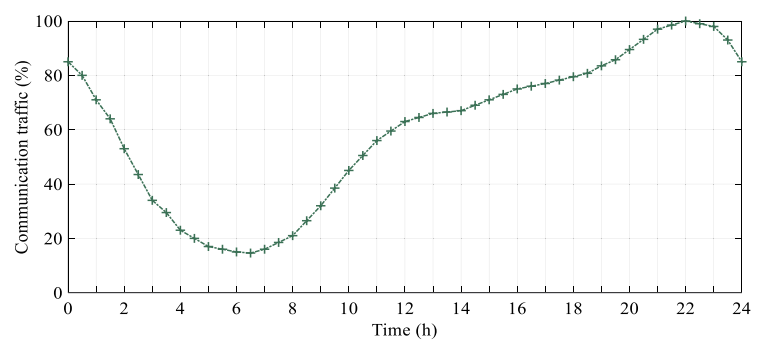
\includegraphics[width=\linewidth]{img/CommTraffic.png}
    \caption{Communication traffic in a heterogeneous cellular network \citep{EnergyOptimization}}\label{subfig:commtrafic}
  \end{subfigure}
  \begin{subfigure}{\linewidth}
    
    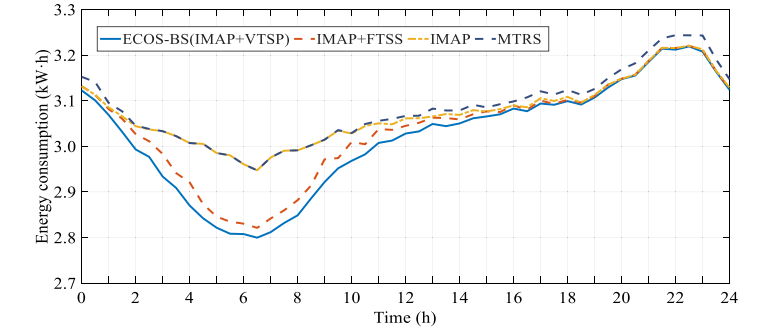
\includegraphics[width=\linewidth]{img/CommTrafficSleep.png}
    \caption{Communication traffic in a heterogeneous cellular network \citep{EnergyOptimization}}\label{subfig:sleepmodes}
  \end{subfigure}
  \caption{}\label{fig:traffic}
\end{figure}

\section{Summary}\label{sec:conclusion}
% Is the situation relevant to national power consumption?
% Are there effective solutions to reduce power consumption?
% Will this topic become more relevant in the future?
% 4 important and relevant indicators of environmental impact: energy consumption, renewable energies, recycling rate and resource productivity
% Germany: 44% renewable energy
% Germany BSs: Maximum power consumption 1.1023146 TWh per year -> 0.224687% of the net national power consumption (0.19234% of production)
% Germany UE: 616.85 GWh per year (382.8996 GWh of that by human-used devices)
% AAU and AC are the biggest power consumers in a BS
% Power consumption cannot be split by component very easily
% Radio cell might range on the same level as the cpu or display by power consumption+
% Giga-MIMO, NR-Light, RedCap NR, NR Sidelink and Sleep modes were presented
% Sleep Modes activation strategies show the greatest potential without introducing new hardware innovation or standards

In this paper, we have delved into the energy footprint of mobile communications in the 21\textsuperscript{st} century, focusing primarily on the context of Germany.
This research reveals several key findings and implications that are worth summarizing and reflecting upon:

\begin{enumerate}
  \item Environmental Footprint: By delineating relevant indicators for environmental footprint assessment, energy consumption and the share of renewable energies have been identified as crucial factors in evaluating the environmental impact of mobile communications.
  The focus on these indicators underscores the need for sustainable energy practices in the mobile communication sector.
  \item Energy Consumption and Production: The national energy data of Germany has been scrutinized  particularly emphasizing the production and consumption of electricity.
  Notably, renewable energy sources have accounted for a significant portion of electricity production, on which mobile communications bases its renewable energy share.
  \item Base Stations: The analysis of base stations underscores their energy demands.
  The distribution of radio systems within base station sites and the average power consumption of \acrshort{aau}s, \acrshort{bbu}s, and \acrshort{ac} units provide insights into their operational dynamics and energy requirements.
  \item User Equipment: Despite challenges in obtaining precise data, an estimation of the power consumption of user equipment has been attempted, considering both human-used devices and \acrshort{m2m} communication devices.
  While uncertainties persist, our analysis sheds light on the overall energy consumption associated with user equipment.
  \item Opportunities for Energy Saving: We have outlined potential avenues for energy conservation in mobile communications infrastructure and devices.
  Strategies such as optimizing power consumption during low-traffic periods, e.g. through the smart usage of sleep modes, and enhancing the efficiency of base station components present tangible opportunities for reducing energy consumption and minimizing environmental impact.
  \item Future Directions: Moving forward, there is a pressing need for continued research and action to address the energy footprint of mobile communications.
  Future studies could explore innovative technologies and policies aimed at further reducing energy consumption, increasing the integration of renewable energy sources, and promoting sustainable practices throughout the mobile communication ecosystem.
\end{enumerate}

In conclusion, This examination of the energy footprint of mobile communications underscores the complex interplay between technological advancements, energy consumption, and environmental impact.
By fostering collaboration among stakeholders and prioritizing sustainability, we can work towards a more energy-efficient and environmentally responsible mobile communication landscape in the 21\textsuperscript{st} century and beyond.

\appendix
\glsaddall
\printnoidxglossary[type=\acronymtype,nonumberlist,style=long]

% \nocite{*}
\renewcommand*{\refname}{\section{References}}
\bibliography{sources}{}
\end{document}
